% *** DOCUMENT CLASS ***
\documentclass{llncs}

% *** MATH ***
\usepackage{amsmath,amssymb,amsfonts}
%\usepackage{theorem}
\usepackage{times}

% *** SUBFIGURE PACKAGES ***
%\usepackage[font={small}]{caption, subfig}
\usepackage[font=footnotesize]{caption, subfig}
\setlength{\abovecaptionskip}{1ex}
\setlength{\belowcaptionskip}{1ex}
\setlength{\floatsep}{1ex}
\setlength{\textfloatsep}{1ex}

% *** FLOAT PACKAGES ***
%
\usepackage{stfloats}

% *** CITATION PACKAGES ***
\usepackage{cite}

% *** GRAPHICS RELATED PACKAGES ***
\usepackage[dvips]{graphicx}
\graphicspath{{figures/}}
\DeclareGraphicsExtensions{.eps}

% *** MISC PACKAGES ***
%
%%% PACKAGE FOR USING THE MULTI-LINE COMMENT
\usepackage{verbatim}
%
%%% COLORS
\usepackage[usenames,dvipsnames]{color}

% *** SETTINGS AND MACROS ***
%% Package to linebreak URLs in a sane manner.
\usepackage{url}
\makeatletter
\def\url@smallurlstyle{%
  \@ifundefined{selectfont}{\def\UrlFont{\sf}}{\def\UrlFont{\small\ttfamily}}}
\makeatother
\urlstyle{smallurl}
\makeatletter
\def\url@tinyurlstyle{%
  \@ifundefined{selectfont}{\def\UrlFont{\sf}}{\def\UrlFont{\scriptsize\ttfamily}}}
\makeatother
\renewcommand{\UrlFont}{\small}
%
%% Make URLs clickable
\usepackage[colorlinks, bookmarks=false]{hyperref}
\usepackage{breakurl}
\hypersetup{ colorlinks=false, citecolor=black,
    filecolor=black, linkcolor=black, urlcolor=black
}

\newcommand\blfootnote[1]{%
  \begingroup
  \renewcommand\thefootnote{}\footnote{#1}%
  \addtocounter{footnote}{-1}%
  \endgroup
}

%
% paper title
% can use linebreaks \\ within to get better formatting as desired
\title{\mbox{GrammarViz\,2.0}: a tool for grammar-based\\ pattern discovery in time series}

\begin{document} 

\author{
Pavel Senin\inst{1} \and 
Jessica Lin \inst{2} \and Xing Wang \inst{2} \and 
Tim Oates\inst{3} \and Sunil Gandhi\inst{3} \and \\ 
Arnold P. Boedihardjo\inst{4} \and Crystal Chen\inst{4} \and Susan Frankenstein\inst{4} 
\and Manfred Lerner \inst{5}}

\institute{University of Hawaii, Manoa, ICS Dept., CSDL, \email{senin@hawaii.edu} \\
 \and George Mason University,
 Dept. of Computer Science, \\
 \email{\{jessica, xwang24\}@gmu.edu}
 \and
 University of Maryland, Baltimore County,
 Dept. of Computer Science,
 \email{oates@cs.umbc.edu, sunilga1@umbc.edu}
 \and
 U.S. Army Corps of Engineers,
 Engineer Research and  Development Center,
 \email{\{arnold.p.boedihardjo, crystal.chen, susan.frankenstein\}@usace.army.mil}
 \and SAP Germany,
 \email{manfred.lerner@sap.com}
}

\maketitle

\begin{abstract}
The problem of frequent and anomalous patterns discovery in time series has received a lot of attention in the past decade. Addressing the common limitation of existing techniques, which require a pattern length to be known in advance, we recently proposed grammar-based algorithms for efficient discovery of variable length frequent and rare patterns. In this paper we present \mbox{GrammarViz\,2.0}, an interactive tool that, based on our previous work, implements algorithms for grammar-driven mining and visualization of variable length time series patterns.\blfootnote{This research is partially supported by the National Science Foundation under Grant No. 1218325 and 1218318.}
\end{abstract}

\section{Introduction}
The ability to efficiently detect frequent and anomalous patterns in time series allows for the exploration, summation, and compression of data. In addition, such information is crucial to a variety of application domains where these patterns convey critical and actionable information, such as health care, equipment safety, and security. Furthermore, these patterns are often used as input features for data mining tasks, such as association rule mining and classification. % \cite{association_rules}

Previously, we defined time series motifs (frequent patterns) \cite{lin_motifs} and time series discords (anomalous patterns) \cite{hot_sax}, and proposed efficient \textit{exact} solutions for their discovery based on Symbolic Aggregate Approximation (SAX) \cite{sax}. While there has been a great amount of follow-up work on the discovery of both pattern types \cite{chan_anomaly}, one common limitation of currently available techniques is that they require the length of a potential motif or discord to be specified as input. This is unreasonable for most real-world problems as such information may not be known in advance, and patterns of different lengths may co-exist in the data.

Addressing this limitation, we recently proposed an alternative solution for the discovery of variable-length motifs \cite{grammarviz} and anomalies \cite{SAXSequitur14} based on SAX discretization and the Sequitur grammar inference algorithm \cite{sequitur}. We showed that our algorithm is able to efficiently discover \textit{co-existing variable-length approximate motifs and anomalies} without any prior knowledge about their length, shape, or minimal occurrence frequency. In this work, we present a time series pattern discovery application called \mbox{GrammarViz\,2.0} that can simultaneously discover variable-length motifs and anomalies. 

\begin{figure}[t]
   \centering
   \includegraphics[width=120mm]{Figure1-ECG0606.eps}
   \caption{An example of a recurrent grammar rule (i.e. \textbf{\textit{motif}}) discovery in the ECG dataset using \mbox{GrammarViz\,2.0}. Note, that the highlighted motif does not cover an anomalous heartbeat and that rule-corresponding subsequences vary in length.}
   \label{fig1}
\end{figure}

\section{Our approach and the tool for time series patterns mining}
Our approach is built on a three phase process: time series discretization, context free grammar induction, and motif/anomaly detection. The first step is to model the time series as discretized elements and convert it into a symbolic representation. The second step is to parse the symbolic series and decompose it into a context free grammar \cite{grammarviz, SAXSequitur14}. Since rules of a context free grammar are hierarchically organized, it is possible to establish the probability of occurrence of a time series subsequence using its corresponding rule hierarchy and rule counts in the entire time series. Intuitively, since each grammar rule represents a discretized subsequence \textit{pattern} of the input time series, frequently used rules are likely to correspond to recurrent subsequences, while infrequently used rules are likely to correspond to rare subsequences. 

Next, we discuss the detailed steps of the above approach and its implementation in our grammar-driven workflow for time series patterns discovery.

\subsection{Dimensionality reduction and discretization with SAX}
Time series are real-valued data whereas grammar induction algorithms are designed for discrete values. We rely on SAX \cite{sax} to discretize the input time series. For time series $T$ of length $m$, SAX obtains a lower-dimensional representation by first performing a \textit{z}-normalization then dividing the time series into $w$ equal-sized segments. Next, for each segment, SAX computes a mean value and maps it to a symbol according to a pre-defined set of breakpoints dividing the data space into $\alpha$ equiprobable regions, where $\alpha$ is the user specified alphabet size. While dimensionality reduction is a desirable feature for exploring global patterns, the high compression ratio ($m/w$) significantly affects performance in cases where localized phenomena are of interest. Thus, for the local pattern discovery, and specifically for motif and anomaly detection, SAX is typically applied to a set of subsequences that represent local features -- a technique called subsequence discretization \cite{lin_motifs} which is implemented via a sliding window. 

Our tool implements both global and local discretization and allows an interactive tuning of discretization parameters using ``SAX parameters'' panel (Fig.\ref{fig1}). In addition, next to the SAX parameters selection, users can toggle the numerosity reduction strategy, which not only mitigates for trivial and degenerate pattern discovery \cite{sax, hot_sax}, but enables an essential feature of our technique -- the discovery of variable-length co-existing patterns \cite{grammarviz, SAXSequitur14}. 

\begin{figure}[t]
   \centering
   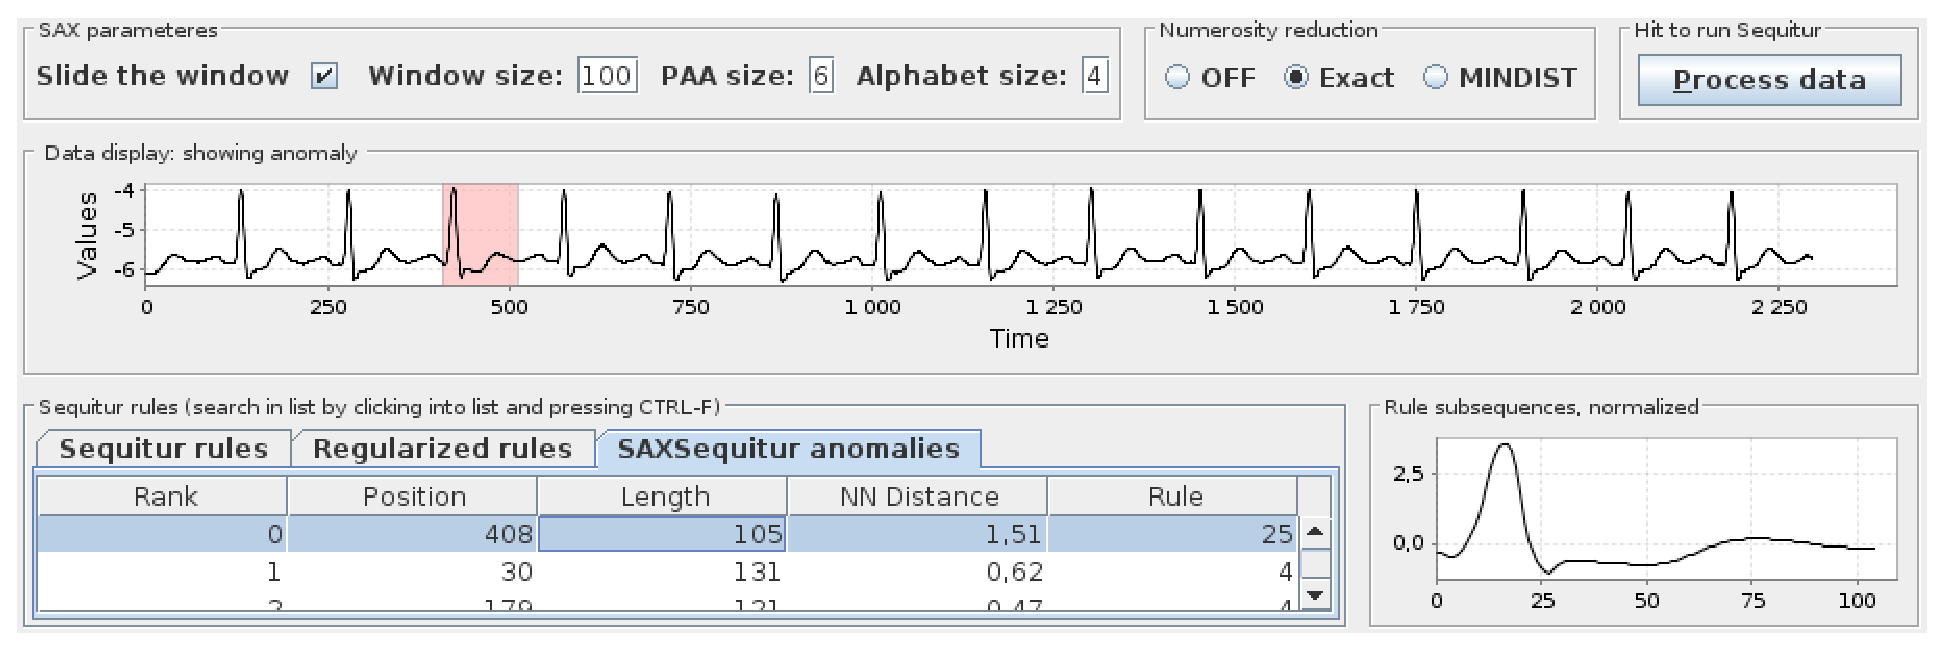
\includegraphics[width=120mm]{Figure2-ECG0606-anomaly.eps}
    \caption{An example of an anomalous grammar rule discovered in the ECG dataset which corresponds to a very subtle anomaly in the ST wave annotated by an expert \cite{hot_sax}.}
   \label{fig2}
\end{figure}

\subsection{Context free grammar induction with Sequitur}
For grammar inference, we rely on Sequitur - a linear time and space algorithm that derives a context-free grammar from a string incrementally \cite{sequitur}. By identifying frequent subsequences in the input string, the algorithm builds a compact context-free grammar reflecting the input string specificity. In addition, we are currently extending our application with mSequitur algorithm implementation that introduces a merging operator and is capable of further grammar reduction by generalization \cite{msequitur}.

Since Sequitur requires no input parameters, in a single ``Process data'' step (Fig.\ref{fig1}) our tool performs both discretization and grammar induction procedures. Once grammar is built, its rules are presented to the user in a table format enabling efficient examination and exploration of rules and their corresponding subsequences. \mbox{GrammarViz\,2.0} shows rule locations on the original time series and superimposes all rule subsequences on a separate panel. This allows visual evaluation of the results from selected parameters as well as their interactive tuning (Fig.\ref{fig1}).

\subsection{Exploiting context-free grammar for pattern discovery}
\textit{\textbf{Motif discovery}}. With the capability to sort the rule table by the rule usage frequency, as well as the effective visual presentation of grammar rules, \mbox{GrammarViz\,2.0} allows user to navigate the rules and visually inspect their corresponding subsequences (``motifs"). \\{\parindent0pt\textit{\textbf{Discord discovery}}. \mbox{GrammarViz\,2.0} enables anomaly detection in two ways: by integrating grammar induction in the HOTSAX discord discovery framework \cite{hot_sax} (Fig.\ref{fig2}), and by visualization of the grammar rule density (Fig.\ref{fig3}). Both approaches allow the user to visually evaluate potential anomalous rules and their corresponding subsequences.

\section{Target Audience and Similar Applications}
As time series are often used as a proxy to represent a large variety of wide ranging real-life phenomena, the \mbox{GrammarViz\,2.0} application targets diverse audiences including researchers, practitioners, engineers, medical specialists, and safety and security personnel. While other time series pattern visualization tools exist \cite{viztree, hao_motifs}, we are not aware of any tool that has the same capabilities as \mbox{GrammarViz\,2.0}; namely, the discovery of hierarchical patterns and variable-length motifs and discords.

\begin{figure}[t]
   \centering
   \includegraphics[width=115mm]{Figure3-ECG0606-density.eps}
   \caption{An example of the ``Data display'' panel showing the ``Rule density'' plot used for highly efficient approximate anomaly discovery through visual examination.}
   \label{fig3}
\end{figure}

\enlargethispage{0.8cm}

\begin{thebibliography}{4}

%1
\bibitem {lin_motifs}
Lin, J., Keogh, E., Patel, P., and Lonardi, S.: 
Finding Motifs in Time Series. 
The 2nd Workshop on Temporal Data Mining, the 8th ACM Int'l Conference on KDD. 53--68, (2002)

%2
\bibitem {hot_sax}
Keogh, E., Lin, J., Fu, A.:
HOT SAX: Efficiently Finding the Most Unusual Time Series Subsequence. 
In Proc. ICDM. 226--233, (2005)

%3
\bibitem {sax}
Patel, P., Keogh, E., Lin, J., Lonardi, S.:
Mining Motifs in Massive Time Series Databases. 
In Proc. ICDM, (2002)

%4
\bibitem{chan_anomaly} 
Chandola, V., Cheboli, D., and Kumar, V.:
Detecting Anomalies in a Time Series Database.
CS Technical Report 09--004, (2009)

%5
\bibitem{grammarviz}
Li, Y., Lin, J., and Oates, T.: 
Visualizing variable-length time series motifs. 
In Proc. of the 2012 SIAM International Conference on Data Mining, 895-906, (2012)

%6
\bibitem{SAXSequitur14}
Senin, P., Lin, J., Wang, X. Oates, T., Boedihardjo, A.P., Chen, C., Frankenstein, S., Gandhi, S.:
Grammar-driven anomaly discovery in time series.
CSDL Techreport 14-05, (2014)

%7
\bibitem {sequitur}
Nevill-Manning, C. and Witten, I.:
Identifying Hierarchical Structure in Sequences: A linear-time algorithm. 
Journal of Artificial Intelligence Research, 7, 67-82, (1997)

%17
\bibitem {jmotif}
Paper authors. Supporting webpage:
\url{http://github.com/GrammarViz2}

\bibitem{viztree}
Lin, J., Keogh, E., Lonardi, S., Lankford, J., Nystrom, D.:
Visually mining and monitoring massive time series. 
In Proc. 10th ACM SIGKDD Intl. Conf. on KDD, 460-469 (2004)

\bibitem{hao_motifs}
Hao, M., Marwah, M., Janetzko, H., Dayal, U., Keim, D., Patnaik, D., Ramakrishnan, N. and Sharma, R. K.:
Visual Exploration of Frequent Patterns in Multivariate Time Series.
Information Visualization, Vol. 11, No. 1, 71-83 (2012)

\bibitem{msequitur}
Oates, T., Boedihardjo, A., Lin, J., Chen, C., Frankenstein, S., Gandhi, S.:
Motif discovery in spatial trajectories using grammar inference. 
In Proc. of ACM Intl. Conf. on Information and Knowledge Management (CIKM) (2013)

\end{thebibliography}

\end{document}